\chapter{Introduction}
\section{The structural design process}
Before a new building or structure can be built it needs to be designed. This design phase, here termed structural design phase, is a very important step of the building process. The total cost for the structure, energy performance, structural performance etc. are largely dependent on the result of the structural design process. 

The structural design process is never a straightforward procedure. Rather, solutions are reached through an iterative, and often chaotic process. The process can be divided in to the four following steps \cite{schlaich2006challenges}:

\begin{enumerate}  
\item Conceiving: The most important design step where the overall design concept and significant details are developed.
\item Modeling: Idealization and simplification of the structural design concept, building of models for structural analysis and calculation of forces.
\item Dimensioning: Deciding sectional dimensions of structural members depending on the choice of materials.
\item Detailing: Final details of nodes and connections including the creation of construction documents.
\end{enumerate}

In reality there is not necessarily a clear distinction between the different design steps and the process can iteratively move forward and backwards until a solution is reached. In this thesis the term conceptual design refers to the first design step conceiving and the initial phase of the modeling step. In the initial design phase the design freedom is considerable. At the same time the impact on the final result of the of the decisions taken at this early stage are often crucial. In contrast, both the design knowledge and the availability of design tools increases as the design matures during the later design stages [2,3], see Figure \ref{fig:freedom-vs-knowledge} and Figure \ref{fig:impact-tools}. The design knowledge comprises of all that is known of the final design, from color of the facade to dimensions of structural members. The lack of tools for the initial design phase combined with the high impact of decisions creates an opportunity to develop such tools. Tools that can support the designer to make well informed decisions in the conceptual design phase.

\begin{figure}
  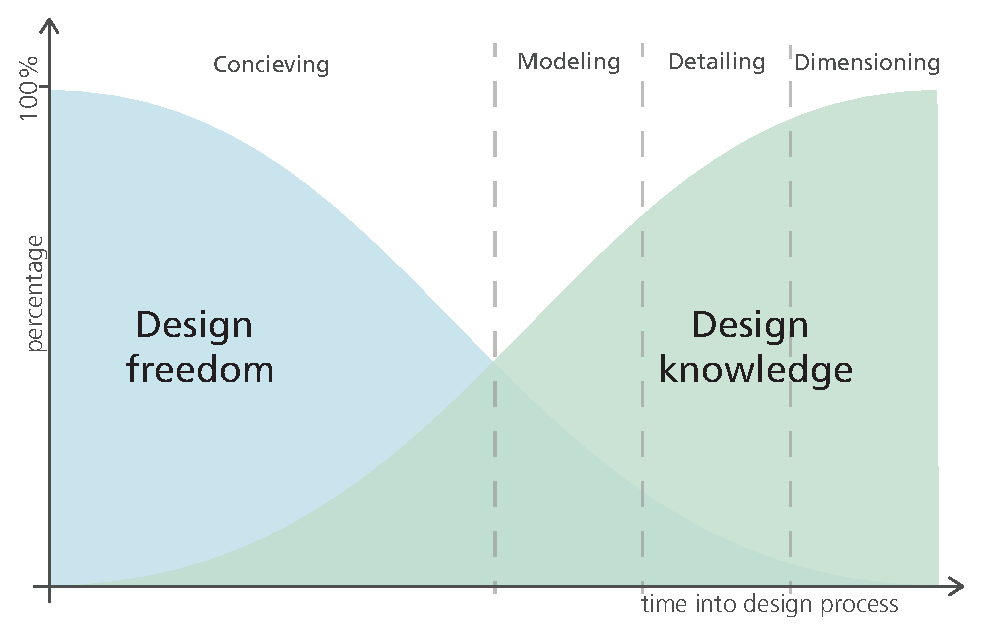
\includegraphics[width=350pt]{graphics/freedom-vs-knowledge.eps}
  \caption{Structural design process \cite{Mueller2014}}
  \label{fig:freedom-vs-knowledge}
\end{figure}

\section{Problem statement}
Many different geometric modeling tools are today available for architects. These geometric modeling tools have, since their introduction in the 1980s, grown increasingly sophisticated. They have also, together with the widespread perception of the benefits of technological innovation, created a more intimate relationship between technology and design. This relationship has resulted in parametric design and scripting methods that can generate complex shapes and forms [4]. The distinct separation found in practice where architect’s use geometric modeling tools and engineers use analysis tools further reinforces the architects role as form-giver and the engineer as form-verifier [5]. To move away from this separation, when the term designer is used in this thesis it represents either an engineer or an architect. Instead of the current practice, it would be beneficial if the engineer and architect would collaborate as designers in the structural design process. This would allow physical demands to work as an inspiration, rather then as a constraint of what is possible, to find new well performing geometric forms. Where physical demands can for example be: structural performance, construction costs, operational energy needs, acoustics.

In the current practice the architect often conceives a design without involvement of the structural engineer. Hence, the importance of the conceptual design phase is often overlooked and structural aspects are often only considered in a late design stage [6]. A contributing factor to this is that very few computational tools are available for conceptual design. 

\begin{figure}
  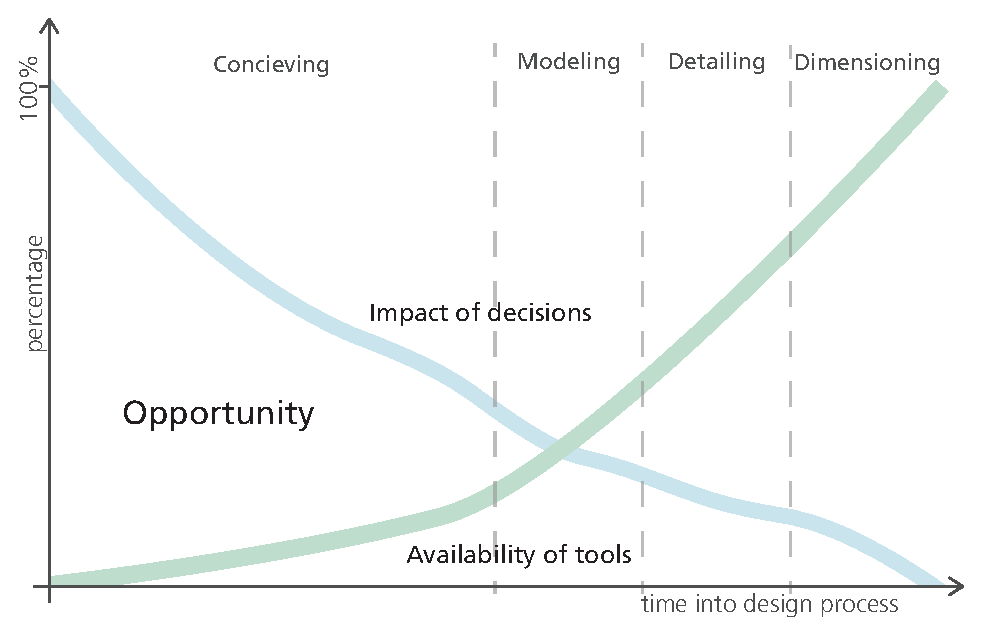
\includegraphics[width=350pt]{graphics/impact-tools.eps}
  \caption{Impact of decisions and availability of tools in the design process [3]}
  \label{fig:impact-tools}
\end{figure}


The challenge when developing such computational tools lies within the fuzzy nature of the problem, knowledge and constraints of the problem are imprecise and incomplete [3].

Conventional advanced structural analysis software requires precise knowledge of the problem and is insufficiently agile to follow a designer’s iterative workflow. Conventional structural analysis software is developed for use in the late design stage, when the major design decisions have been made, as a tool for the engineer to verify the form. 

A subsequent problem with the traditional workflow, where the architect is the form-giver and the engineer is the from-verifier, can arise due to the availability of the a very detailed geometric model. It can be tempting for the engineer to directly perform a full analysis on the detailed geometry something which is possible with today’s structural analysis software. If instead the engineer starts with a simple mathematical model and then gradually increases the complexity - known as hierarchical modeling, see Figure \ref{fig:hiarchical-modelling} – the risk of fatal mistakes is decreased [7]. 

By starting with a simple mathematical model the engineer can focus on, and get a better understanding of, the overall structural behavior. Where the overall structural behavior is how stresses follow through the structure, what the magnitude of the stresses are in different structural members, etc. This information can be valuable when a more advanced mathematical model is used, to confirm the feasibility of the results. It has been shown that premature use of advanced structural analysis software negatively affects the conceptual understanding and the quality of the conceptual design [8].

In the present work, two similar computational conceptual design tools have been developed. The two applications make use of simple mathematical models, which enables structural modeling to be used earlier in the structural design process. The motivation for this is two-fold. It can give the designer valuable feedback on structural performance in the conceiving phase, when the impact of decision still is high. And it can also give the engineer valuable feedback on structural behavior before a more advanced model is used. 

\begin{figure}
  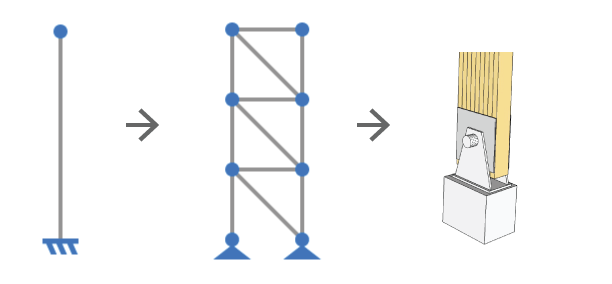
\includegraphics[width=310pt]{graphics/hiarchical-modelling.png}
  \caption{Hierarchical modeling}
  \label{fig:hiarchical-modelling}
\end{figure}

The type of design tool that is used to generate and represent ideas also affects the quality and quantity of early prototypes. It was shown in [9] that physical prototyping generated a higher quantity of prototypes, compared to using CAD or conventional sketching, under the same amount of time. The prototypes that were developed using physical prototyping were also perceived as more novel compared to the other prototypes. However, the prototypes that were perceived as more novel also tended to fare poorly on all other measureable qualities [9]. 

In the present work the prototypes are structural models. As computational models are used, a measurable performance can be computed and presented to the user in real-time. This can potentially can improve the quality of the structural models. The measureable performance and guidance in the present work put emphasis on the geometrical form of the structure as this has the greatest potential to improve the structural performance [10]. 

\subsection{Examples of well-executed conceptual structural design}
Structural demands can be integrated earlier in the design process by using them as inspiration of geometric forms instead of constraints of what is possible. Integrating structural demands earlier in the design process have the potential to reduce the amount of material needed, reduce environmental impact and lower costs for the project as a whole \cite{Mueller2014}. 

\begin{figure}
  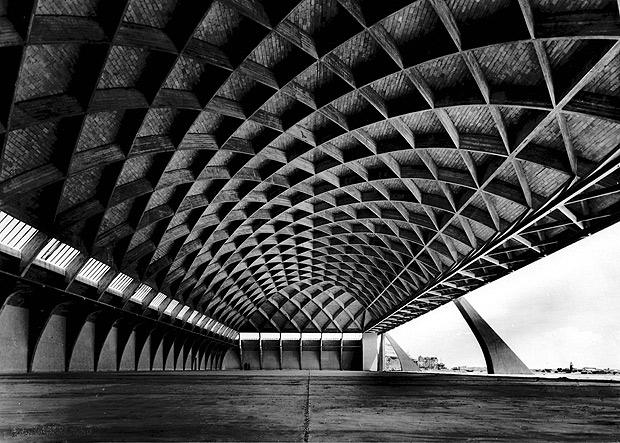
\includegraphics[width=350pt]{graphics/nervi.jpg}
  \caption{Pierre Luigi Nervi - Air hangar, built 1936}
  \label{fig:nervi}
\end{figure}

A good example of well-executed conceptual designs are the structures designed by the Italian architect-engineer Pierre Luigi Nervi, see example in Figure \ref{fig:nervi}. Despite the complexity of his structures his designs were often selected because they were the cheapest to build [11], as less material was needed for his designs compared to his competitors. This type of complex concrete structure is unfeasible when labor costs are high, due to the extensive formwork required [12]. However, This is something which could of course change in the future with the emergence of robots and digital manufacturing [13].

“His buildings are most remarkable for the clarity of their engineering. The power and grace of these extraordinary shapes and patterns stems directly from their structural logic, and are inseparable from it” – Ada Louise about Pierre Luigi Nervi, 1960 \cite{Mueller2014}

The Shenzhen CITIC Financial Center, see Figure \ref{fig:Shenzen}, is a more recent example of well-executed integrated conceptual design. The perimeter frames are inspired by research on optimal discrete truss geometries to minimize the material needed [14].

\begin{figure}
  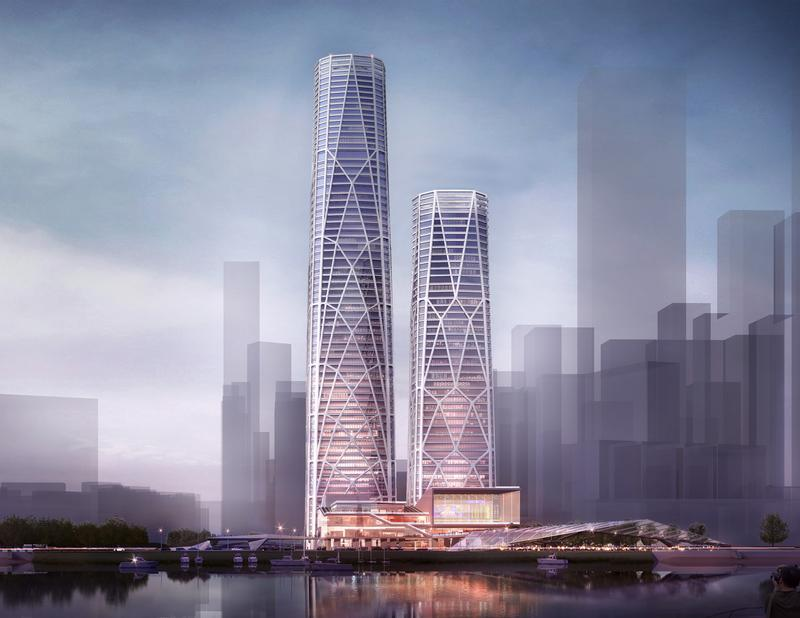
\includegraphics[width=350pt]{graphics/shenzen.jpg}
  \caption{Shenzen CITIC Financial Center, Lead Architectural Partner: Craig W. Hartman, Lead Structural Partner: Mark Sarkisian.  Rendering © Skidmore, Owings \& Merrill LLP, 2016}
  \label{fig:Shenzen}
\end{figure}

Designing Nervi’s air hangar in 1936 required a very thorough understanding of structural mechanics. He was at the time the only one, or one of very few engineers that was capable of successfully designing such a structure. The CITIC Financial center was also designed by a team distinguished designers. The difference between the two examples are that the latter used computer computations in the design process. 

\subsection{Computational design tools}
Computational design tools have the possibility make computer computations readily available in the design process, to help guide the designer towards well-performing solutions. Such tools have previously been developed and a review of existing tools and the methods that they implement are available in Chapter 3. These tools are developed to follow the designer’s iterative workflow, which the conventional structural analysis software lacks. 

Allowing these computational tools to follow the designer’s iterative workflow puts high demand on the user interface of the tools. Most of the existing computational design tools are developed for mouse and keyboard input. In the present work alternative input devices are explored, which allows for a more direct input. 

\section{Research methodology }
\subsection{Aim of research}
The long term goal with this research is to improve the conceptual design phase by integrating structural demands early in the design process. An improved conceptual design phase has the potential to improve the quality of structures in the built environment. These qualities can for example be: structural performance, construction costs, operational energy needs, acoustics.


\begin{itemize}  
\item To improve conceptual structural design by developing computational tools that bridge the gap between the design steps conceiving and modeling.
\item  To create intuitive conceptual structural design tools that allow the user to easily explore different design alternatives.
\item To improve the human-computer interaction for such tools though use of new, novel user input devices. 
\end{itemize}


\subsection{Research questions}
\begin{itemize}  
\item How can the human-computer interaction be improved in computational conceptual structural design tools?
\item  Which computational methods can be used to improve the conceptual design phase? 
\end{itemize}

\subsection{Research approach and limitations}
The present research is a multi-disciplinary work between structural mechanics, computer science and architecture. Methods from structural mechanics are used to provide the user with guidance and feedback. Developing user interfaces and employing programming techniques is a part of the computer science discipline. Studying conceptual design and finding geometrical forms are a part of architecture. The research is applied and any successful tools that this work results in could potentially be used in practice with few changes.

There are different research approaches to investigate how the conceptual structural design phase can be improved. In this work, it has only been investigated how new computational tools can improve the conceptual design phase. Project management, social aspects and culture is not considered in this work.

Many different computational methods exist that can be used for conceptual structural design. Some promising methods are presented in Chapter 4, a selection of these methods have been used in the present work.

\subsubsection{Outline}
Part I is an introduction to the research area and also literature review of previous work in this field. This part is similar to, but an extension of, the introductory sections in the appended papers. Chapter 1, is an introduction to the research area, and motivates why this work is important. Chapter 2 introduces human-computer interaction to the reader and introduces state of the art technology, such as new input devices. Chapter 3, presents computational methods that can be applied to conceptual design. Different optimization methods, especially the genetic algorithm, are thoroughly introduced; as these methods will be used in future work. Chapter 4 reviews existing conceptual structural design tools. In Chapter 5 the developed applications are presented, and the publications that this work has resulted in are presented in Chapter 6. Chapter 7 summarizes the present work and the intellectual contributions.





%%%%%%%%%%%CHAPTER 2%%%%%%%%%%%%%%%%

\Chapter{Human-computer interaction}
Human-computer interaction is a multi-disciplinary research area that includes: user interface design, hardware, software, social aspects and more. Important concepts in this research area are usability and user experience.

With new technology such as novel input devices and increased computational power comes new possibilities. The present work makes use of these new possibilities. Novel user input devices are used for structural modeling, and increased computational power is used for real-time structural analysis. 

\section{Direct manipulation}
Direct manipulation is a human-computer interaction style with continuous representation of objects of interest with rapid, reversible and incremental feedback [15]. Users can directly manipulate objects on the screen using real-world metaphors, which makes the users more engaged with their task and encouraged to further explorations [16]. This is achieved through reducing the perceptual and cognitive resources required to understand and use the user interface [17].

\subsection{Visualizations}
Scientific visualization is a subfield of computer graphics. The purpose of scientific visualizations is to graphically illustrate scientific data. This is also important for any conceptual structural design software to be successful, how the result is visualized is of great importance. The result should be visualized in a way so that the user quickly can interpret the result and gain insight from it. 


Figure 6 Visualization of how a car deforms in an asymmetrical crash using finite element analysis.

In Figure 6 is an example of how the result from a computational analysis often is performed. The original geometry, an undeformed car, is modified with the computed displacement. The geometry, in this case the car, is also colored according to some selected condition. The color can for example represent von Mises tensions, shear forces, bending moment etc. 



Edward Tufte is one of the pioneers in the field of data visualization with his books on information design [18–20]. He has in [20] written a few principles of graphical excellence which he stated as follows:



\item Graphical excellence is the well-designed presentation of interesting data – a matter of substance, of statistics and design.

\item Graphical excellence consists of complex ideas communicated with clarity, precision and efficiency.

\item Graphical excellence in that which gives to the viewer the greatest number of ideas in the shortest time with the least ink in the smallest space.

\subsubsection[1.1.3 Technology]{1.1.3 Technology}
The introduction of different input devices such as the mouse and joystick significantly improved the human-computer interaction of user interfaces that adapted accordingly [17]. When the touch screen was introduced it had an advantage over all these devices. The user could literally touch objects on the screen to manipulate them, creating a very direct method of inputting information[17]. This closed the gap between the human and the computer.



There is a wide repertoire of interaction techniques to create direct manipulation user interfaces for 3D applications using 2D input devices such as the mouse [21]. However, since this type of input devices have one degree of freedom less than the 3D user interface there will always exist a need of gestures or similar methods. 



The Leap Motion controller [22], is a relatively small and simple input device that is placed in front of the users keyboard, it then tracks the users hands that are in the controllers field of vision. Combined with the software development kit (SDK), the controller creates a computational model of the users hands, which can then be used to interact with software in 3D. This enables very direct manipulations for 3D user interfaces.



Computer games have seen an increase in the amount of novel input devices along with a new style of games to address some limitations of conventional systems [23], e.g. the Wii remote [24], Microsoft’s Kinect for Xbox [25] and PlayStation Move [26]. These novel input devices move away from the conventional human-computer interaction to invoke an intuitive interaction that supports the natural human way of working. Games have for long been perceived as fun and engaging, and it has been investigated in many different disciplines if gaming methods can improve the human-computer interaction. In order to create more effective, immersive and engaging learning or training [23]. 



Interest for and development of virtual reality glasses have recently increased, and products such as the Oculus Rift [27] and PlayStation’s Project Morpheus [28], have recently become widely available. This type of virtual reality glasses has primarily been developed for games but other fields have also shown interest, e.g. in [29] a virtual reality is used to help students understand complex structural behavior.



\section{Computational methods}
In this section a number of computational methods that can be used for conceptual structural design are introduced. 

\subsubsection[1.1.4 Form Finding]{1.1.4 Form Finding}
Physical models or numerical simulations can be used for form finding, where the aim is to find the form for a structure under load where static equilibrium is satisfied. The static equilibrium corresponds to a structure that can support the applied load using only compression or tension, thus a very efficient structure. For physical models a hanging chain or cloth can be used the find the static equilibrium.



A number of different form finding methods exists, and they can be divided into three major categories [30]: 

\item Stiffness matrix methods - which are based on elastic and geometric stiffness matrices. These methods have adapted methods structural analysis for form finding.

\item Geometric stiffness methods - these methods are material independent. The first such example is the force density method [31] which makes use of the ratio of force to length. Several other methods have been developed which extends on this work.

\item Dynamic equilibrium methods {}- these methods find the steady-state equilibrium through use of dynamics. One such method is dynamic relaxation [32] which is explained in further detail in Section 3.1.1.1.





Figure 7 Funicular shapes by Stevin (1586)

\paragraph[1.1.4.1 Dynamic relaxation]{1.1.4.1 Dynamic relaxation}
Dynamic relaxation is a method to solve a set of non-linear equations. The method computes the movement of a structure over time to find static equilibrium between the internal and external forces [32,33]. 



In each time step,  
 , for all elements are computed from the nodal displacements u. A residual, R, can be computed by using 



 is the external forces acting on the structure. By using Newton’s second law the acceleration (time derivative of the velocity) can be computed as follows (at the node i, in the x-direction, at the time t)


 is a lumped, fictitious mass at node i. To enforce boundary conditions, the residual is set to zero for the corresponding degrees of freedom. With the time step known the velocity of node i in the x-direction can be computed using finite difference method

With the velocity known the updated geometry can now be updated by using

As the geometry is updated, an iteration is complete and the computations start over, by again, computing the residual. The geometry is modified in each iteration until equilibrium between external and internal forces has been reached. Viscous or kinetic damping is often used in order for the method to converge [33].



A recent development is a formulation that combines CAD-geometry and dynamic relaxation [34] for form-finding.









\subsubsection[1.1.5 Optimization methods]{1.1.5 Optimization methods}
Michell was a pioneer in the field of structural optimization [35] when he in 1904 published his results with minimum-weight Michell trusses. These trusses are still used today as benchmarks for topology optimization with framed trusses [36]. 



Structural optimization is a numerical method to find the best solution for a mathematically formulated objective function that is subject to a set of constraints. The following variables are always present in structural optimization [37]:

\item Objective function (f) {}- A function to classify designs from a quantifiable objective, the function returns a numerical value that represents how good the design is out of one or more criteria. Usually a small number is better then a large, i.e. a minimization problem. Frequently f measures weight, maximum displacements, strain energy or cost.

\item Design variable (x) – A vector that describes the design with numerical values, it often represents a topology, nodal positions, cross sectional area or material.

\item State variable (y) – For a given design with the design vector x, y represents the response of the structure i.e. how well the structure is performing from the evaluated criterion.



The optimization problem can now be described as follows [37] :



 A number of different numerical methods exist to perform the optimization, and the best method depends on the solution space for the problem.



A problem can also have multiple objective functions, so called multi-objective optimization. Which can be formulated as follows:


This is not a standard optimization problem as the objective functions are optimized for the same design variables. Instead a so-called Pareto optimality is sought, where there is no other design that satisfies all the objectives better [37]. If no single Pareto optimal point exists instead a Pareto front can be found in the objective space, where the objective space is a space with the different objectives on the axis. The objects can for example be, structural efficiency, operational energy consumption, sunlight etc.

\paragraph[1.1.5.1 Gradient based methods]{1.1.5.1 Gradient based methods}
Gradient-based methods make use of the first, and some the second, derivative to iteratively converge towards a solution. These types of methods are fast, consistent and the result is repeatable (no randomness). However, the solution space of the objective function needs to be convex (such as the design space in Figure 8), continuous and at least once differentiable. The problem with using this type of methods for engineering and design, is that the problems are often so-called messy problems [2], that is non-convex solution spaces that contain multiple local optima. Examples of gradient-based methods are steepest descent and Newton-Rhapson [37]. 

Figure 8 Design space for a shape optimization problem

\paragraph[1.1.5.2 Evolutionary algorithms]{1.1.5.2 Evolutionary algorithms}
Evolutionary algorithms are a collection of generic population-based heuristic optimization algorithms [38]. The algorithms are inspired by biological evolution, survival of the fittest and natural selection. The solvers introduce randomness to search the solution space, which improves the algorithms ability to find the global optima.



One of the most well-known and used algorithms in this category is named genetic algorithm [39], it is inspired by the biological evolution. The benefits of this algorithm are that it is very robust and always returns a solution and the objective function does not need to be differentiable. 

Figure 9 Genetic Algorithm procedure

The procedure for genetic algorithm can be described as follows, see Figure 9:



\item Create initial population – First an initial population is created, either on random or through some type of sampling (e.g. Latin hyper sampling [40]).

\item Evaluate fitness of each individual – The objective function is called which gives each individual a score (heuristic).

\item Apply selection – The individuals with a high fitness score have a higher chance to by selected for crossover, a biological metaphor for mating.

\item Crossover/Mutation – The individuals with a high fitness recombine properties (in this context design variables) with each other, to create a new generation. Introducing a small chance of mutation, a random change, when two individuals crossover can minimize the risk of the algorithm to get trapped in local optima. Elitism can be introduced to always allow the best performing individuals to move to the next generation, which can improve convergence. 

\item End – The procedure continues until a preselected criterion is reached, often number of generations or when solution stops to converge.



A weakness of genetic algorithm is that it can be very computationally heavy, as the objective function needs to be called for each new individual. There is also a lot of fine tuning, different types and rates of crossovers, mutations etc. 



A strength of the algorithm is that multiple well performing solutions can be presented fore the user (different individuals from the population). This can be used in conceptual design, where an aesthetically attractive well-performing solution is sought. The algorithm can also be used for interactive optimization [41], where a user can intervene the selection process to move the population in a desired direction. The algorithm has also been adjusted for use with multiple objective optimization, where the population converges to the Pareto front [42].



\paragraph[1.1.5.3 Topology optimization]{1.1.5.3 Topology optimization}
To optimize the material layout, given a set of boundary conditions and external forces, topology optimization can be used. The method can be implemented through the use of finite element analysis combined with optimization methods [43]. However, the resulting optimal material layout can be infeasible to build due to high complexity.

\subsubsection[1.1.6 Eigenvalue analysis]{1.1.6 Eigenvalue analysis}
Eigenvalue analysis can be used to find the dynamic or static modal shapes for a structural model. From the stiffness matrix K of a structure, a set of scalar stiffness values can be determined [44]. Assume that a set of displacements a exists, that are proportional to a corresponding set of forces f, i.e.


This can be combined with a linear elastic finite element formulation, i.e.

This is a standard eigenproblem. The eigenvalues   

 have the unit force/length, also called canonical stiffness values [45]. Every eigenvalue  

 has a corresponding eigenvector   

 , which describes a modal shape. Eigenvalues equal to zero means zero energy is required to form the corresponding modal shape, i.e. a rigid body motion. The eigenvectors are only defined within a scalar multiple. To create an animation of the modal shape, the eigenvector can be normalized and multiplied with a positive and negative scalar. This result in two different shapes, interpolation between the two shapes can then be used to create an animation.



\subsubsection[1.1.7 Graphic statics]{1.1.7 Graphic statics}
Graphic statics is a graphical method to find funicular shapes and compute forces for structural models through the use of a force diagram. The method was first published in 1886 by Karl Culmann [46], the method was widely used until the 1970s, when the increase in computational power made numerical simulations widely available. 



The method has recently gained attention from the research community [12,47,48] because of its simplicity and power. However, the method is limited to statically determinate problems with axially loaded members. 



\section{Literature review}
\subsection[1.2 Analysis{}-based tools for engineers]{1.2 Analysis-based tools for engineers}
The development of finite element analysis (FEA) has resulted in many different, but very similar, software analysis tools. These tools are often too complex and not agile enough to be used for conceptual design. Their use requires a high level of skills both in connection with the software and in engineering terms. This type of software has been developed for the late design stage as a tool for the engineer to verify the form. 

 The analysis procedure for this type of software is often a step-by-step workflow, where all the steps need to be completed in order before the analysis is carried out, see Figure 10. The user experience has been compromised by this step-by-step evolution.


Figure 10 Conventional simulation cycle

Figure 11 User interface of conventional analysis software (ABAQUS)

\subsection[1.3 Geometry{}-based tools for architects]{1.3 Geometry-based tools for architects}
\subsubsection[1.3.1 History]{1.3.1 History}
The first computer-aided design (CAD) tool, termed Sketchpad [49], was developed by Ivan Sutherland at MIT in 1963. The revolutionary feature of Sketchpad was real-time representation of the geometry on the display, which could be modified with the use of a new input device, a light pen. The light pen enabled a complete interaction loop between the computer and the designer. The software had support for complex relationships between graphical elements; for example, a line could be defined by relationship to other graphical objects, perpendicular to, parallel to, same length etc. Sutherland had a vision that the designer would first create a rough sketch of the design. And then, as the design matured, apply constraints to the graphical objects to get a more detailed and precise design. 


Figure 12 Sketchpad - the first CAD tool

Computer aided design tools, 2D drafting tools, were first affordable and accessible to a wider audience in the 1980s [49]. The succeeding 2D drafting software unfortunately failed to capture Sutherland’s original intentions of using the computer as a creative design tool, by not including the constraint model. 

\subsubsection[1.3.2 Present day]{1.3.2 Present day}
As mentioned earlier, many different geometric modeling tools are today available for designers, such as parametric modelers. These parametric modelers have successfully captured some of Sutherland’s ideas of constraint models. 



The software Rhinoceros 3D [50], which is a NURBS modeler, can be combined with the plug-in Grasshopper [51], that enables a visual programming environment, see Figure 13. The software developer company Autodesk has also launched a parametric modeling tool named Dynamo [52] that has similar features.


Figure 13 The parametric modeling tool Grasshopper

In Grasshopper the designer can connect a slider to a parameter - for example the width or curvature of a model – the geometry then updates in real-time as sliders are manipulated. This enables complex shapes and forms to be generated and manipulated, allowing the designer to explore the parametric design space. 



Many plug-ins also exist for Grasshopper, and these can be combined with each other, one such example is Karamba [53], which enables structural performance feedback within the parametric modeler. 

\subsection[1.4 Existing conceptual design tools]{1.4 Existing conceptual design tools}
“Geometry and algorithms can exist in the abstract, but to be of any practical significance, to become a design tool which can be used by designers, then these have to be encapsulated in an executable form, as working software…” - Robert Aish [54]

A number of different conceptual design tools exist; they have here been divided into categories depending on the computational methods that they make use of.



\subsubsection[1.4.1 Real{}-time analysis tools]{1.4.1 Real-time analysis tools}
This type of conceptual design tools makes use of simple mathematical models to provide the user real-time feedback from structural analysis. Various such tools have previously been developed, the first two such tools were developed in parallel and released in 2006, named Pointsketch [45] (see Figure 14) and Arcade [55]. In the two different software tools, the user can create a structural model using mouse and keyboard input. Forces can then be applied to the model and the results are visualized in real-time 



The first tools were developed in academia but industry has shown interest in the concept. Autodesk launched a new application in 2011 named ForceEffect [56], which is available both as an tablet and as a web application. The application is developed for designers to analyze and visualize two-dimensional truss structures. The tablet application utilizes a direct manipulation user interface style where the user can make changes to the model by directly touching the objects. The commercial finite element (FE) software SAP2000 [57] launched in 2012 a model alive feature, this feature enables real-time feedback with deformations and forces for truss-structures [58].


Figure 14 The software tool PointSketch

Recently an interactive physics engine was developed to create a user experience inspired by games for design and education [59]. The developed physics engine has been used to create an interactive game called Catastrophe, which aims to teach users which elements are critical to system stability through play.


Figure 15 The interactive graphic statics software Equilibrium [47] 

Multiple graphic static computational design tools have been developed; they make use of graphic statics simplicity that allows the computations to run in real-time.



The first developed such application is ActiveStatics [60], a web-based tool that allows the user to explore graphic statics. Focus of the tool is teaching how graphic statics works, and extensive examples are available. A very similar version named Equilibrium [47] was later developed, see Figure 15. Another similar design tool that instead makes use of particle-spring system for computations is CADenary [61].


\subsubsection[1.4.3 Interactive optimization design tools]{1.4.3 Interactive optimization design tools}


Figure 16 Screenshot of StructureFIT

Genetic algorithm can easily be used for interactive optimization, where the user can intervene the selection process and direct the population in a desired direction. Such applications have been developed for conceptual structural design, to generate and analyze structures such as bridges and trusses. One such tool is von Buelow’s interactive evolutionary design tool [62], which has support for both 2D and 3D structures.

Another similar application, developed as a web application, is named StructureFIT [63,64], see Figure 16. The software tool also has a direct manipulation mode where the user can further explore a generated structure by moving nodes and in real-time see how a relative performance index is updated. Another version of this tool has been developed for Grasshopper [51], named Stormcloud [65].


\subsubsection[1.4.4 Topology optimization design tools]{1.4.4 Topology optimization design tools}
Two other applications that were developed in academia for design exploration through the use of topology optimization are ForcePad (see Figure 17) [66] and TopOpt [67]. In the two applications a 2D geometry is modeled by use of conventional drawing tools, a metaphor for “drawing with stiffness”. A topology optimization is then performed on the geometry and the resulting optimized shape is visualized. The applications also have an interactive mode where forces can be manipulated, and the resulting stresses updated in real-time.


Figure 17 Software tool ForcePad


%%%%%%%%%%%%%NEW CHAPTER%%%%%%%%

\section{Integrating structural feedback in conceptual design tools}
In the conventional workflow the architect uses geometric modelling tools and the engineer deploys structural analysis tools in a sequential step. Parametric modeling tools are an improvement to this workflow, as structural analysis plug-ins are available. This allows the user to get structural feedback earlier in the design phase, but still as a sequential step to the geometric modeling.



The present work purposes an improvement to the workflow by integrating structural feedback with geometric modeling. However, this creates new demands on conceptual design tools. 

\subsection[1.5 Human{}-computer interaction]{1.5 Human-computer interaction}
The conceptual design tools should inspire and encourage the user to explore design alternatives. This puts demands on the human-computer interaction of such tools. The tools need to be interactive and allow the user to, quickly create new models, or to make changes to existing models. 



Direct manipulation is a human-computer interaction style that enables the user to directly manipulate objects on the screen, and by doing so, reducing the perceptual and cognitive resources required to understand and use the user interface. In Paper 1, a conceptual design tool has been created which employs a very direct manipulation user interface for 2D. This is achieved by taking advantage of the multi-touch screen – which literally closes the gap between human and computer. In this work, the user can input a structural model by using gestures similar to those found in drawing applications for tablets, see Figure 18. This allows the user to quickly explore different design alternatives.



  [Warning: Image ignored] % Unhandled or unsupported graphics:
%\includegraphics[width=3.3752in,height=2.6354in]{../../Library/Group%20Containers/UBF8T346G9.Office/msoclip1/01/clip_image040.png}
 

Figure 18 Modelling gestures in the developed application Sketch a Frame



Achieving a very direct manipulation in 3D is today possible with the emergence of new 3D input controllers. This creates an opportunity to create conceptual design tools with a very direct manipulation for 3D. In Paper 2, this opportunity has been explored by developing a conceptual design tools which employs a very direct manipulation for 3D. This has been achieved by using a 3D input controller named the Leap Motion Controller. 



In Paper 1, a very direct manipulation cycle is purposed which further improves interactivity of the user interface of conceptual design application. As the user is modelling, computations are continuously performed, and when the modeled structure is stable the result is automatically visualized. This removes the need for a specific “compute step” which further integrate structural feedback into the geometric modelling. This direct manipulation cycle is also employed in the developed application in Paper 2.

\subsection[1.6 Structural feedback]{1.6 Structural feedback}
To integrate structural feedback into conceptual design applications structural analysis must be integrated with the geometrical modeling. The feedback should also be easy to understand and provide valuable feedback of the structural behavior and performance.

In the developed applications in Paper 1 and Paper 2, an external force can be applied to the modeled structure. If the model is stable – the resulting deformations can be visualized in real-time. The user can then manipulate the force using direct manipulation, and in real-time see how the structural deformation responds. In Paper 1, when an external force has been applied, the resulting normal forces and the moment envelope can also be visualized in real-time. This can improve the user’s understanding of, how the structure responds to external forces - how stresses follow through the different members, and the stiffness of the structure in different directions.



The structural feedback should be easy to understand for the user. In Paper 2, a model can be manipulated by the previously described direct manipulation methods, simultaneously the user is presented with a performance index, which is a measure of how well performing the structure is. The performance index is the normalized strain energy of the model; thus a lower number means a better performing structure, see Figure 19. Presenting a single number that represents how well performing the structure is makes it easy for the user to understand how geometrical modifications affects the structural performance.



  [Warning: Image ignored] % Unhandled or unsupported graphics:
%\includegraphics[width=3.3752in,height=2.4689in]{../../Library/Group%20Containers/UBF8T346G9.Office/msoclip1/01/clip_image042.png}
 

Figure 19 Geometric modeling with real-time performance index

\subsection[1.7 Structural optimization]{1.7 Structural optimization}
Integrating structural optimization into conceptual structural design has the possibility to not only give feedback of the structural performance but also to guide the user towards geometries that are structurally well performing. 



A genetic algorithm has been implemented in the application described in Paper 1, which can be used for shape optimization. The user first selects which nodes and in which direction (vertical or horizontal) that the optimizer is allowed to move the nodes. Then the optimization can be executed and the strain energy is minimized. After the analysis is complete the best performing structure is visualized, see Figure 20. 

  [Warning: Image ignored] % Unhandled or unsupported graphics:
%\includegraphics[width=3.3752in,height=2.1457in]{../../Library/Group%20Containers/UBF8T346G9.Office/msoclip1/01/clip_image044.png}
 

Figure 20 Genetic algorithm optimization in Sketch a Frame

Form finding can be used to find the static equilibrium for a structure under load. In Paper 2, the dynamic relaxation method has been implemented to enable form finding in an interactive 3D environment. The user can further explore the form found structure by applying and manipulating an external force. The point load can here be used to move away from the optimal solution in order to find other interesting sub optimal solutions that might be more aesthetically attractive to the user. The point load can also, for example, represent a supporting column or a hanging installation in the structure.



\subsection[1.8 Visual representations]{1.8 Visual representations}
After structural analysis computations have been performed the result can be visualized. For conceptual structural design tools, visualization where the user can quickly get an understanding of the results are sought. 



One such example is graphostatics, which visualize forces as lengths of lines in the force diagram. This is beneficial for the users understanding, compared to using colors to represent the size of the forces, as it removes a layer of abstraction. The user can directly understand the size of the forces without the need of a for example a colorbar.



To visualize dynamic behavior animations can be used. This is used in the application developed in Paper 1 – if a force is applied to a non-stable model the corresponding mechanism is visualized by using an animation. This allows the user to quickly understand the model’s non-stable behavior, and how the model needs to be modified in order to make it stable. 

\subsubsection[1.8.1 Example {}- Loadpaths]{1.8.1 Example - Loadpaths}
Structural behavior of 1D elements, such as bar and beam elements, are easier to understand than higher dimensional elements. Higher dimensional elements have a more complex structural behavior. For 2D structural elements the internal stresses can be computed and used to compute lines which represents how the external load flows through the structure towards the boundary conditions. Here described for the Z-direction [70]:



  [Warning: Image ignored] % Unhandled or unsupported graphics:
%\includegraphics[width=1.25in,height=0.2709in]{../../Library/Group%20Containers/UBF8T346G9.Office/msoclip1/01/clip_image045.png}
 





The author has explored how loadpaths can be extended into 3D by using volumetric elements. The idea for the algorithm is explained in Figure 20.



  [Warning: Image ignored] % Unhandled or unsupported graphics:
%\includegraphics[width=2.948in,height=3.6043in]{../../Library/Group%20Containers/UBF8T346G9.Office/msoclip1/01/clip_image047.png}
 

Figure 20 Computing loadpaths for 3D

The method has been used to produce Figure 21, where the volumetric elements are colored according to the von Mises stress and the green dots are boundary conditions. However, this method does have some drawbacks; it is unclear how to interpret the lines, sensitivity to the mesh and computational heavy. Also, only the internal stresses acting in the Z-direction are here considered.

  [Warning: Image ignored] % Unhandled or unsupported graphics:
%\includegraphics[width=3.3854in,height=1.3854in]{../../Library/Group%20Containers/UBF8T346G9.Office/msoclip1/01/clip_image049.png}
 

Figure 21 Loadpath visualized using in 3D for Z-direction

